\chapter{Chapter with number}
\section{그림과 표를 본문에서 이야기하기}

본문에서 그림과 표에 관해 이야기를 할 때도 인용에서처럼 하시면 됩니다.

%% Table in a separate file
%%
%% 표 삽입 예시
%% Example. how to insert table
%%
\begin{table}[t]
\caption[캡션제목 넣으십시오]{표 제목을 넣으십시오.
}
\label{mag-tab1}
\begin{center}
\begin{tabular} {ccccccccccc}
\hline\hline
& & BF &\multicolumn{2}{c}{SW-I}&&\multicolumn{2}{c}{SW-II}&SW-III&CAP&\\
\cline{4-5} \cline{7-8}
&               &   &  Para & Ferro &&   Para &  Ferro &      &      &\\
\hline
& $E$ (eV)      & 0 & 7.796 & 7.832 && 10.418 & 10.408 & 11.5 & 13.2 &\\
& $M$ ($\mu_B$) & 0 &     0 &  1.94 &&      0 &   2.06 &    0 &    0 &\\
\hline\hline
\end{tabular}
\end{center}
\end{table}
 %Path viewed from top directory


%%
%% 그림 삽입 예시
%% Example. how to insert graph
%%
%% Note. 가급적 \includegraphics 명령을 사용하십시오.
%% Recommen : Use \includegraphics to insert graph.
%%
\begin{figure}[t]
    \centerline{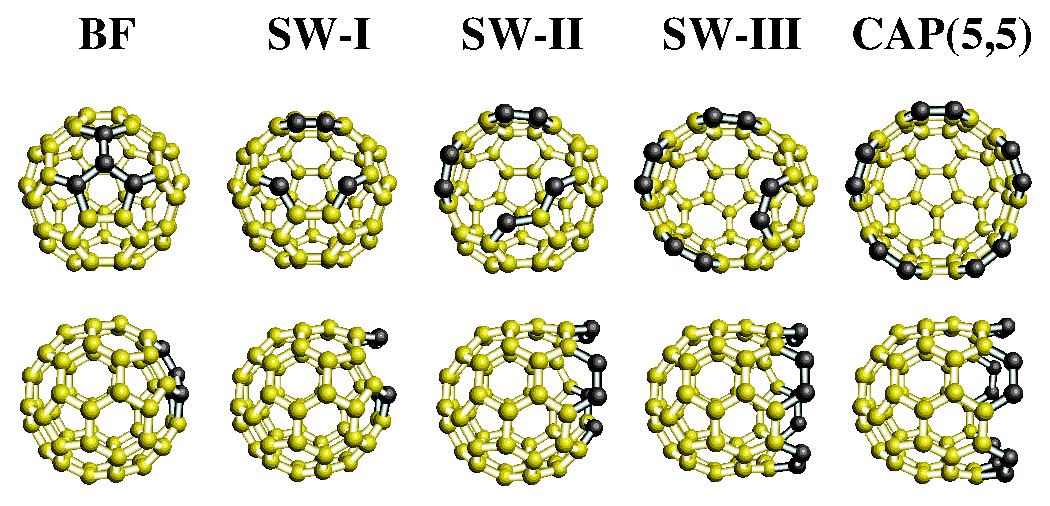
\includegraphics[width=12.5cm]{figures/sample-fig1}} %Path viewed from top directory
    \caption[캡션제목 넣으십시오]{그림 제목을 넣으십시오.
    } \label{mag-fig1}
\end{figure}
